















% \begin{figure*}[htbp] 
% 	\begin{center} 
% 		\includegraphics[width=0.99\linewidth]{figures/comparison1.jpg} 
% 	\end{center} 
% 	\vspace{-16pt}
% 	\caption{Qualitative comparison with SOTA playback-only methods on novel view synthesis on DualGS dataset.}
% 	\label{fig:fig_comp_1}
% \end{figure*} 


% \begin{figure*}[htbp] 
% 	\begin{center} 
% 		\includegraphics[width=0.99\linewidth]{figures/comparison2.jpg} 
% 	\end{center} 
% 	\vspace{-16pt}
% 	\caption{Qualitative comparison with AP-NeRF~\cite{uzolas2024template}, TAVA~\cite{li2022tava} and SC-GS~\cite{huang2024sc} on both training motion and novel motion synthesis.}
%         \vspace{-16pt}
% 	\label{fig:fig_comp_2}
% \end{figure*} 


\section{Experimental Results} 

\subsection{Quantitative Comparison: Task 2 vs. Task 3}
\begin{figure*}[t]
    \centering
    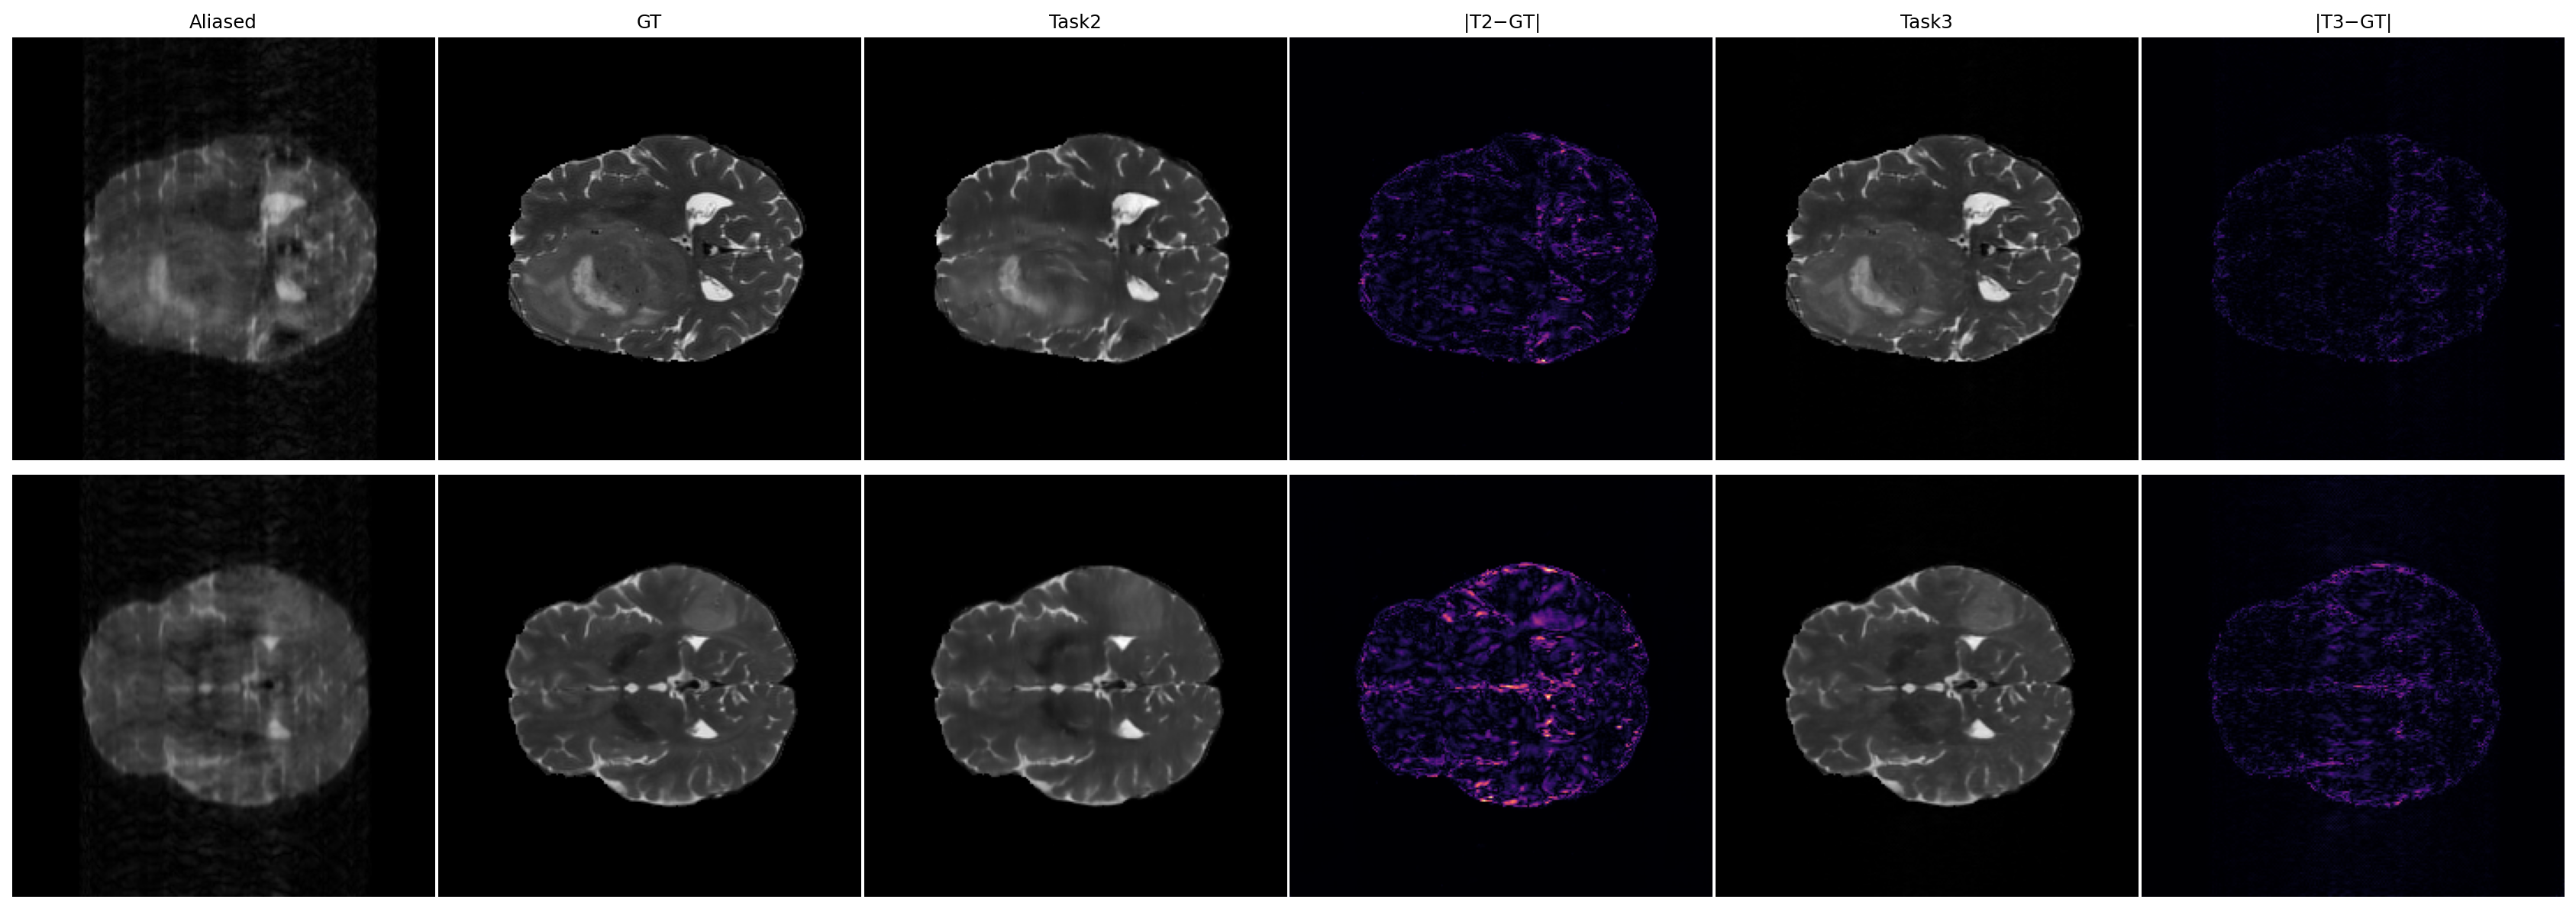
\includegraphics[width=\textwidth]{figures/task2_task3_two_case_paper_grid.png}
    \caption{Qualitative comparison of reconstruction results between Task 2 and Task 3.}
    \label{fig:qualitative_results}
\end{figure*}

To comprehensively evaluate the reconstruction performance of the baseline U-Net (Task 2) and the proposed Multi-modal Unrolled Network (Task 3), we adopted four complementary metrics, including Peak Signal-to-Noise Ratio (PSNR), Structural Similarity Index Measure (SSIM), Learned Perceptual Image Patch Similarity (LPIPS), and Deep Image Structure and Texture Similarity (DISTS). While PSNR and SSIM mainly measure pixel-level fidelity and structural consistency, LPIPS and DISTS further evaluate perceptual similarity and texture preservation from a human visual perspective.

As summarized in Table~\ref{tab:main_results}, the proposed Task 3 framework consistently achieves superior performance across all evaluation metrics. Specifically, Task 3 improves PSNR from 37.21 dB to 41.11 dB and increases SSIM from 0.885 to 0.954, demonstrating substantially better reconstruction accuracy and structural consistency. Meanwhile, LPIPS decreases from 0.0205 to 0.0090 and DISTS decreases from 0.1558 to 0.0936, indicating that the proposed method produces reconstructions with significantly improved perceptual quality and more realistic texture recovery.

The qualitative comparisons in Figure~\ref{fig:qualitative_results} further support these observations. Compared with the baseline Task 2 results, the Task 3 reconstructions exhibit sharper anatomical boundaries, clearer tumor structures, and fewer residual artifacts. Moreover, the corresponding error maps ($|T2-GT|$ and $|T3-GT|$) reveal that the proposed method significantly suppresses reconstruction errors, particularly around fine structural details and high-frequency regions. These improvements demonstrate the effectiveness of incorporating multi-modal priors together with iterative data consistency refinement in the unrolled reconstruction framework.

\begin{table}[h]
\centering
\caption{Quantitative comparison between Task 2 (Baseline) and Task 3 (Multi-modal Unrolled Network).}
\label{tab:main_results}
% 将表格宽度缩放为当前行宽 (列宽) 的 90%。高度设为 ! 表示保持原本的长宽比。
\resizebox{1.0\linewidth}{!}{
\begin{tabular}{lcccc}
\toprule
\textbf{Model} & \textbf{DISTS} $\downarrow$ & \textbf{LPIPS} $\downarrow$ & \textbf{PSNR} $\uparrow$ & \textbf{SSIM} $\uparrow$ \\
\midrule
Task 2 (U-Net) & 0.1558 & 0.0205 & 37.21 & 0.885 \\
Task 3 (Proposed) & 0.0936 & 0.0090 & 41.11 & 0.954 \\
\bottomrule
\end{tabular}
}
\end{table}

\subsection{Qualitative Results and Training Logs}

Figure~\ref{fig:random_sampled_worst_distinct_patients_paper_figure} shows the five worst Task 3 cases ranked by PSNR. Despite severe aliasing in the inputs, the reconstructions preserve the main anatomical structures and lesion regions, demonstrating the robustness of the proposed model on challenging samples. Remaining errors mainly appear as mild over-smoothing of fine textures and residual boundary artifacts, especially near cortical folds, tumor margins, and image borders.

Figure~\ref{fig:training_logs_1} shows the validation curves of the Task 2 baseline. The validation loss and NMSE decrease rapidly in the early training stage and then gradually converge, while PSNR and SSIM increase and stabilize. This indicates that the baseline U-Net learns a reasonable reconstruction mapping from undersampled inputs. However, the PSNR and SSIM curves exhibit noticeable early-stage fluctuations, suggesting that the baseline remains less stable on challenging validation samples.

Figure~\ref{fig:training_logs_2} further reports the Task 3 training dynamics. The training and validation losses decrease rapidly in the early epochs and then gradually stabilize, suggesting effective optimization without obvious overfitting. Meanwhile, PSNR increases steadily, while LPIPS and DISTS decrease, indicating simultaneous improvements in pixel fidelity, perceptual similarity, and structural texture preservation.

Overall, the qualitative results and training logs are consistent with Table~\ref{tab:main_results}. Task 3 produces sharper and more faithful reconstructions than the Task 2 baseline, while the remaining failures are mainly concentrated in fine anatomical details, lesion boundaries, and image-edge artifacts.

\begin{figure}[h]
    \centering
    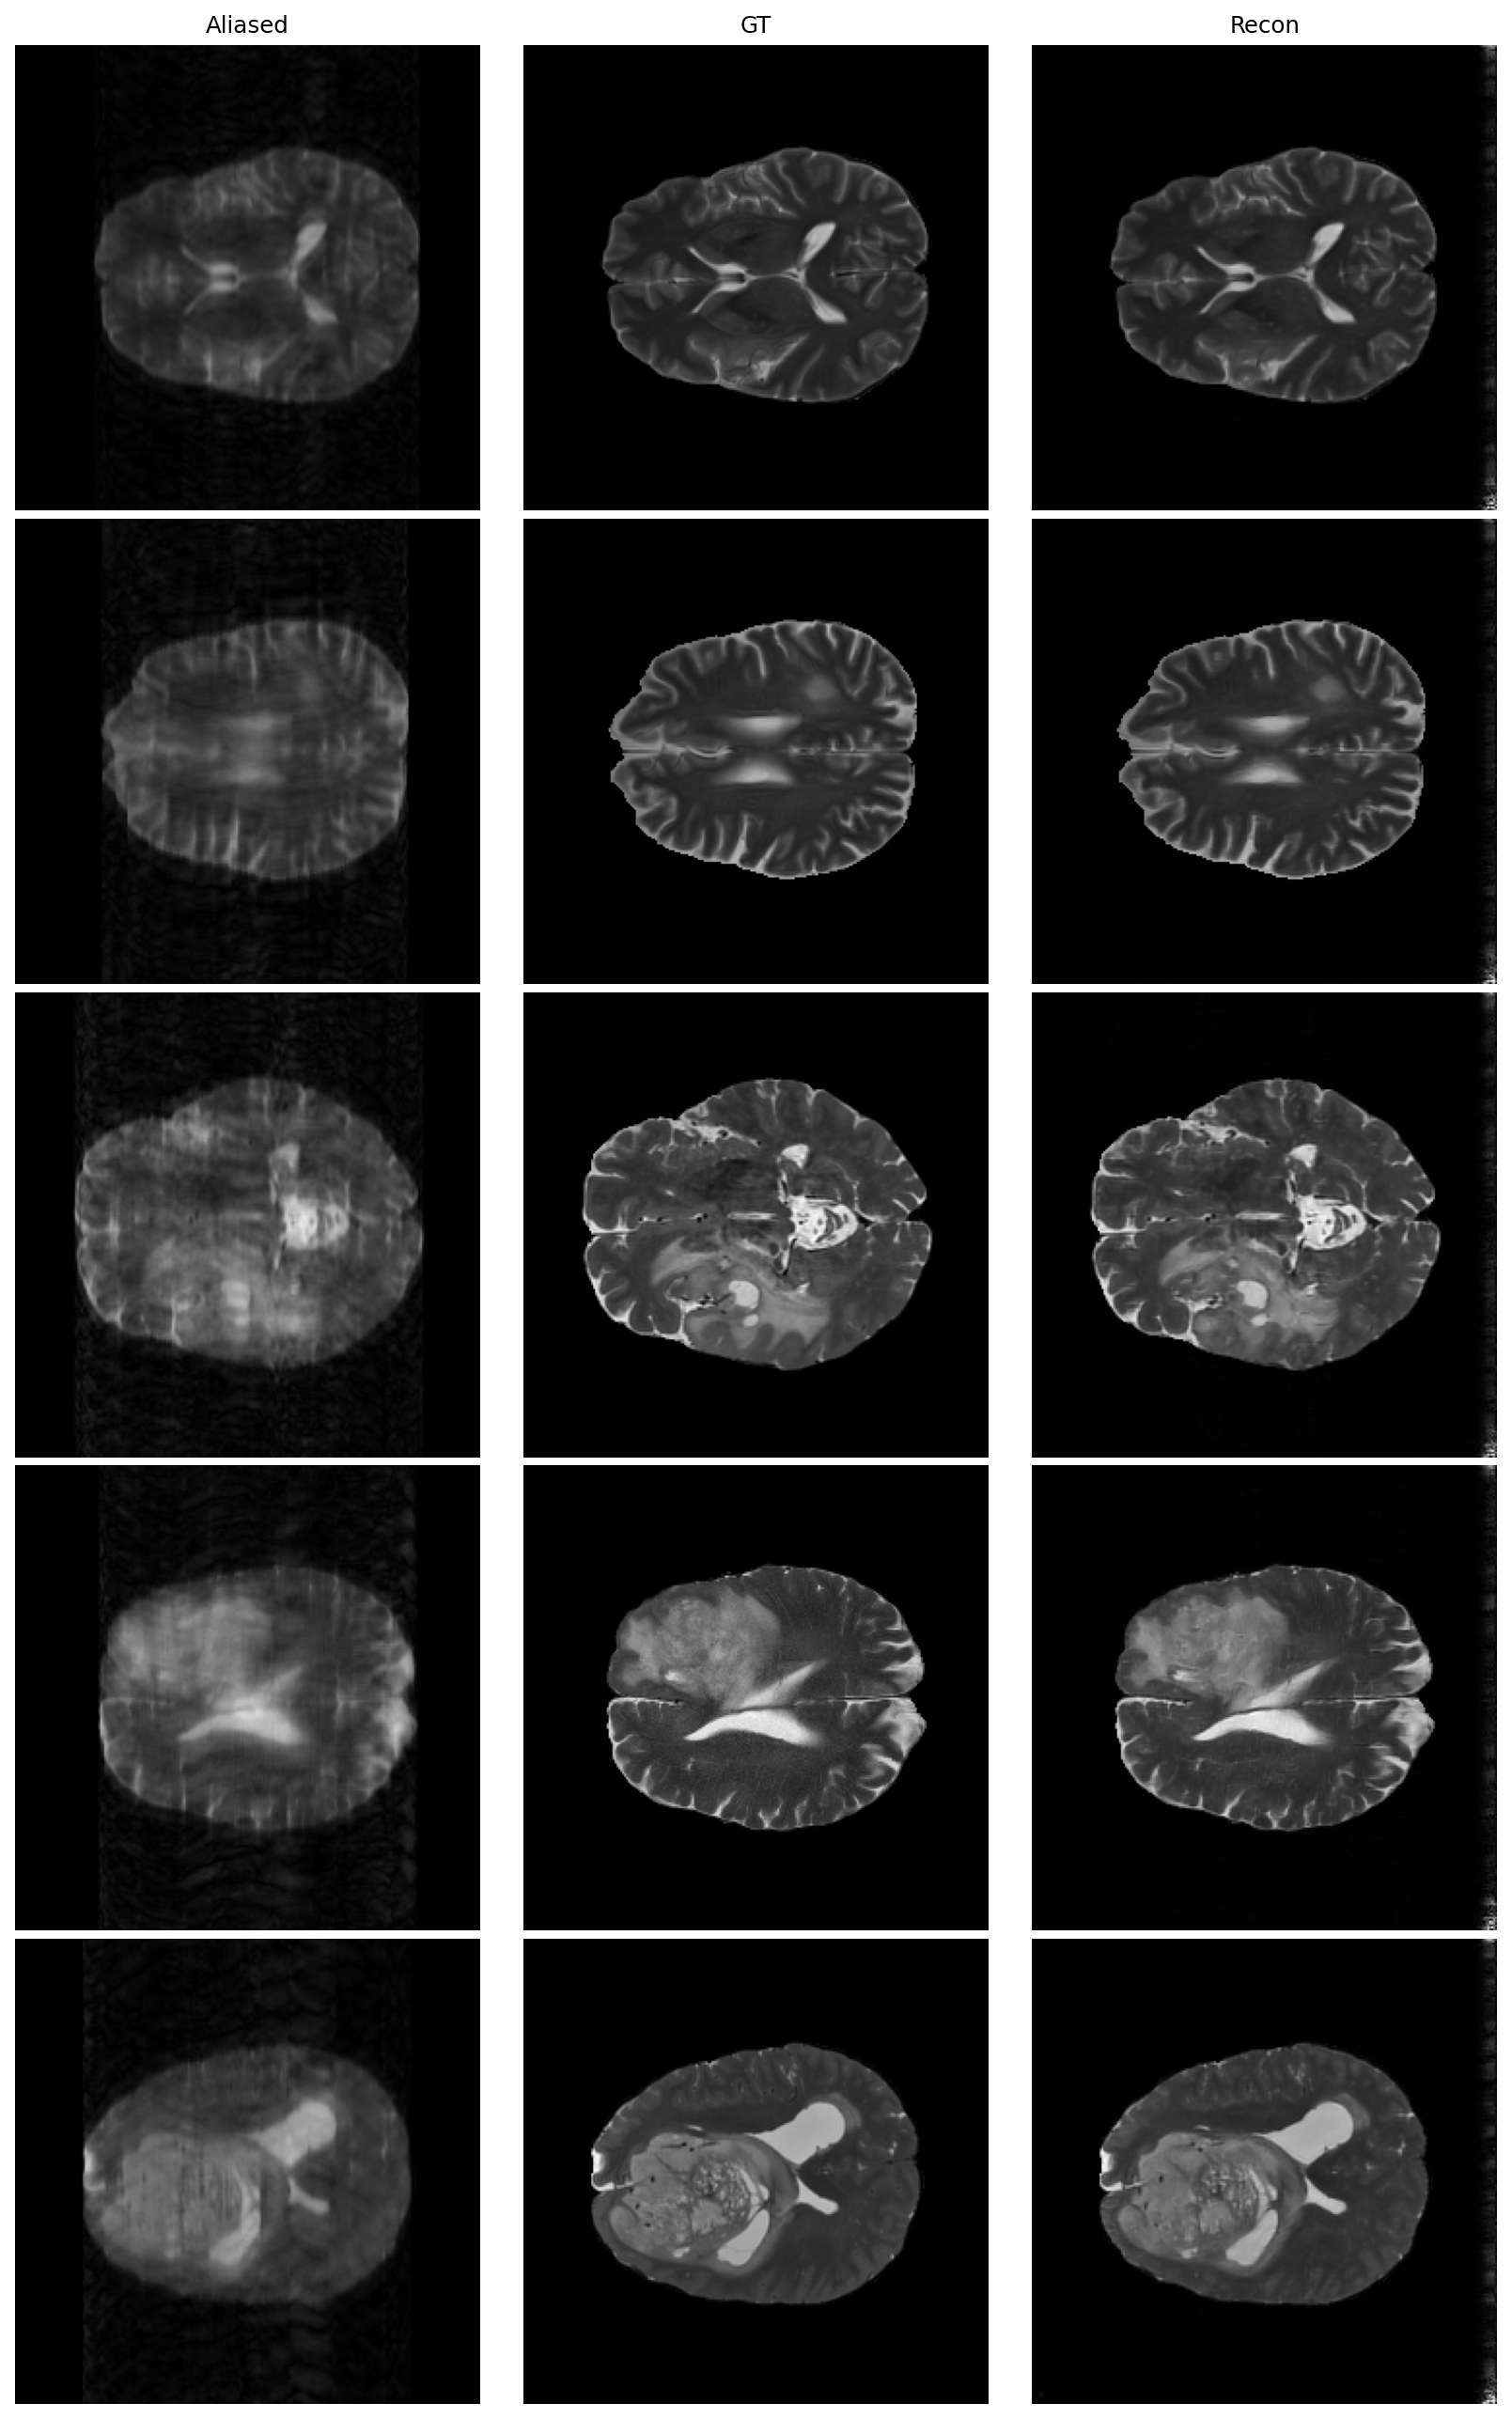
\includegraphics[width=\linewidth]{figures/random_sampled_worst_distinct_patients_paper_figure.png}
    \caption{The five worst-performing reconstruction cases from the task3 baseline (calculated using PSNR as the metric).}
    \label{fig:random_sampled_worst_distinct_patients_paper_figure}
\end{figure}

\begin{figure}[h]
    \centering
    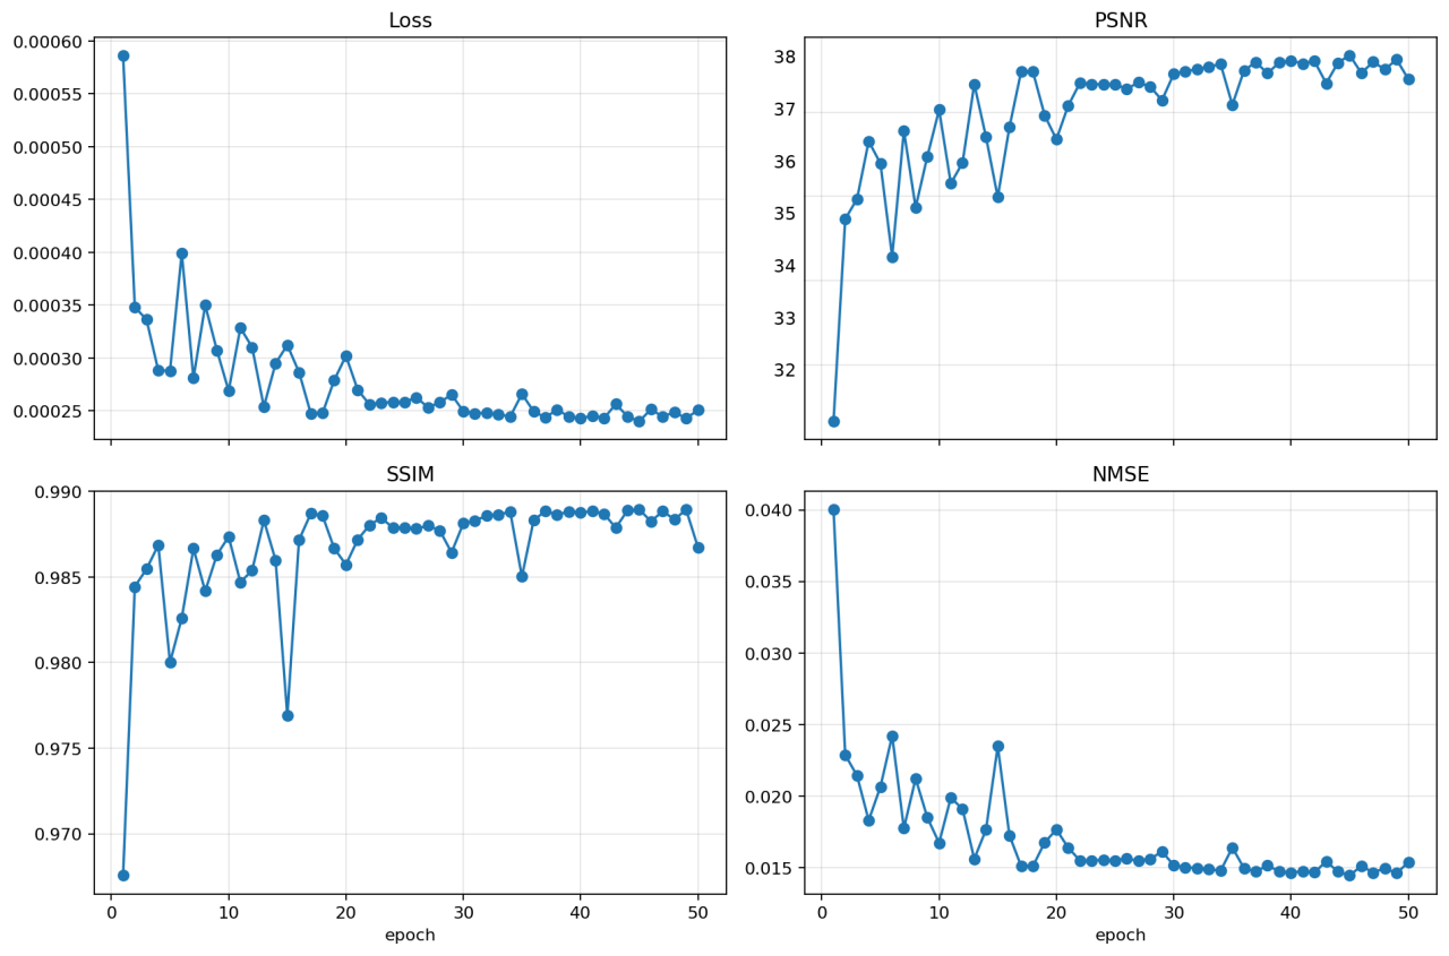
\includegraphics[width=\linewidth]{figures/training_logs_1.png}
    \caption{Validation loss curves for Task 2.}
    \label{fig:training_logs_1}
\end{figure}

\begin{figure}[h]
    \centering
    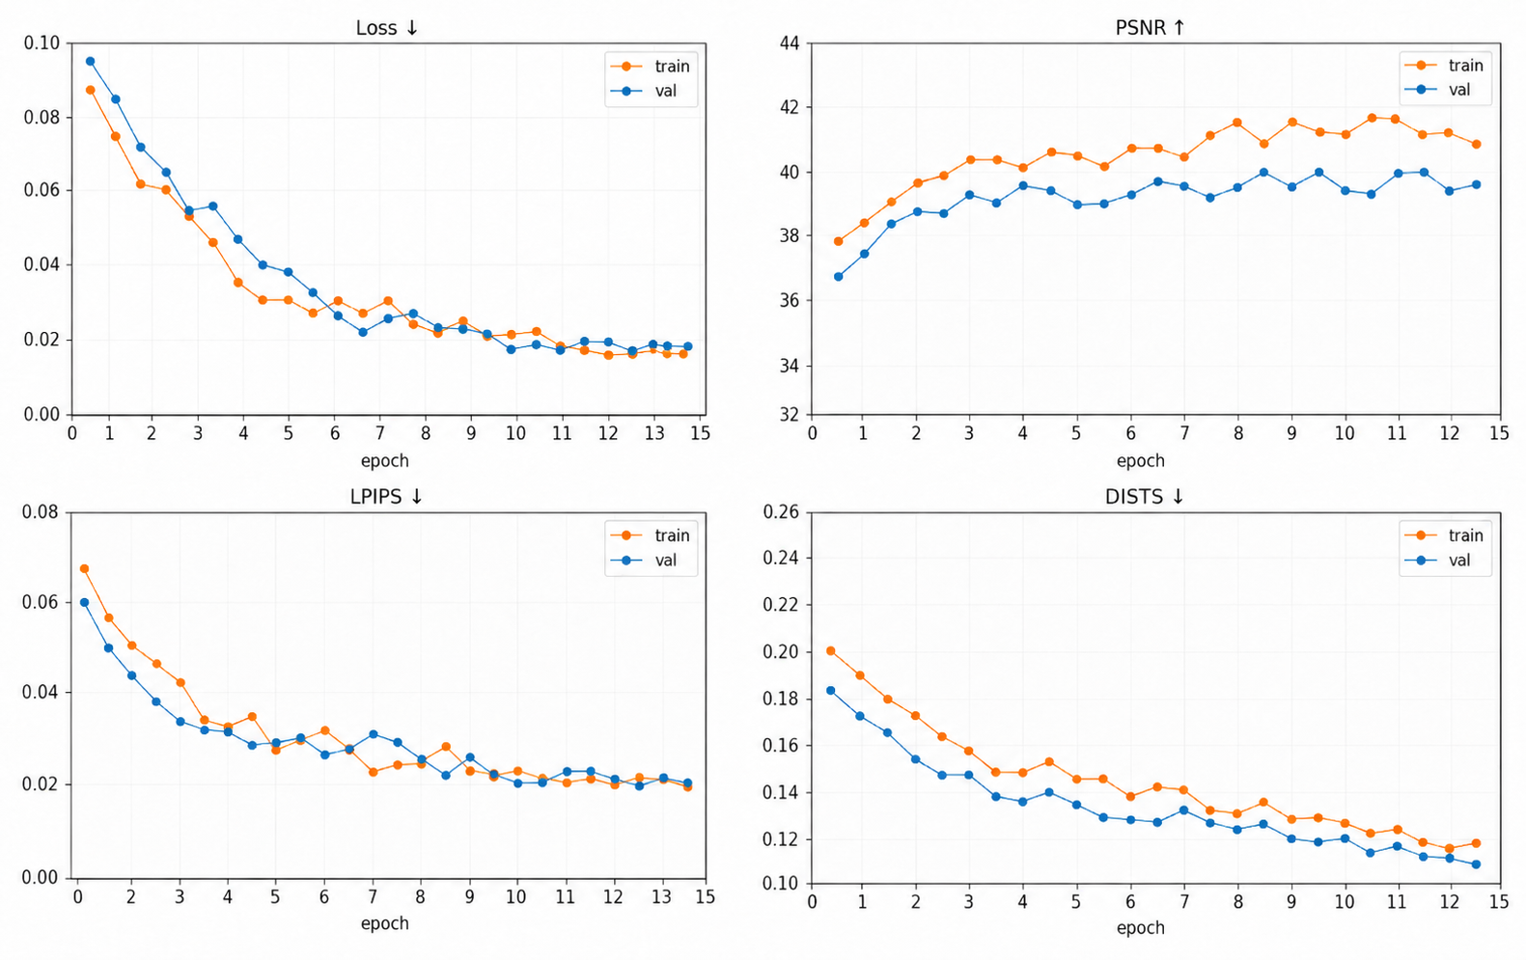
\includegraphics[width=\linewidth]{figures/training_logs_2.png}
    \caption{Training and Validation loss curves for Task 3.}
    \label{fig:training_logs_2}
\end{figure}

\subsection{Rethinking PSNR: Alignment with Human Perception}
During our initial analysis of the Task 2 results, we encountered a significant contradiction: images with higher PSNR values did not consistently yield better subjective visual quality. As illustrated in Figure \ref{fig:psnr_error}, Slice 43 achieves a higher PSNR (39.10 dB) than Slice 28 (35.34 dB). However, inspecting the Error Maps and the perceptual LPIPS metric reveals the opposite story: Slice 43 has a significantly worse LPIPS score (0.0364 vs. 0.0194) and exhibits denser, more structured errors, aligning better with human visual dissatisfaction.

\begin{figure}[h]
    \centering
    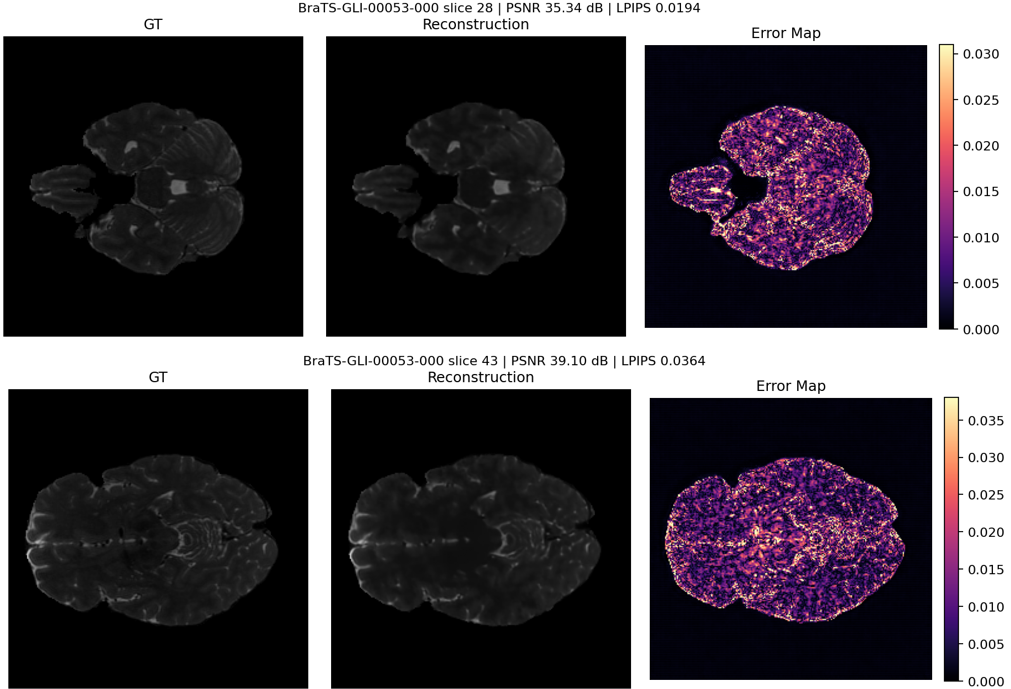
\includegraphics[width=\linewidth]{figures/PNSR.png}
    \caption{Contradiction between PSNR and Perceptual Quality. Slice 43 (bottom) has a higher PSNR but a noticeably worse Error Map and LPIPS score compared to Slice 28 (top).}
    \label{fig:psnr_error}
\end{figure}

To systematically investigate this metric failure, we drew inspiration from the supplemental materials of Apple's research on image sharpness \cite{mescheder2025sharp}. We conducted a ``shifting pixels'' experiment by translating the reference MRI image by minor spatial percentages. 

\begin{figure}[h]
    \centering
    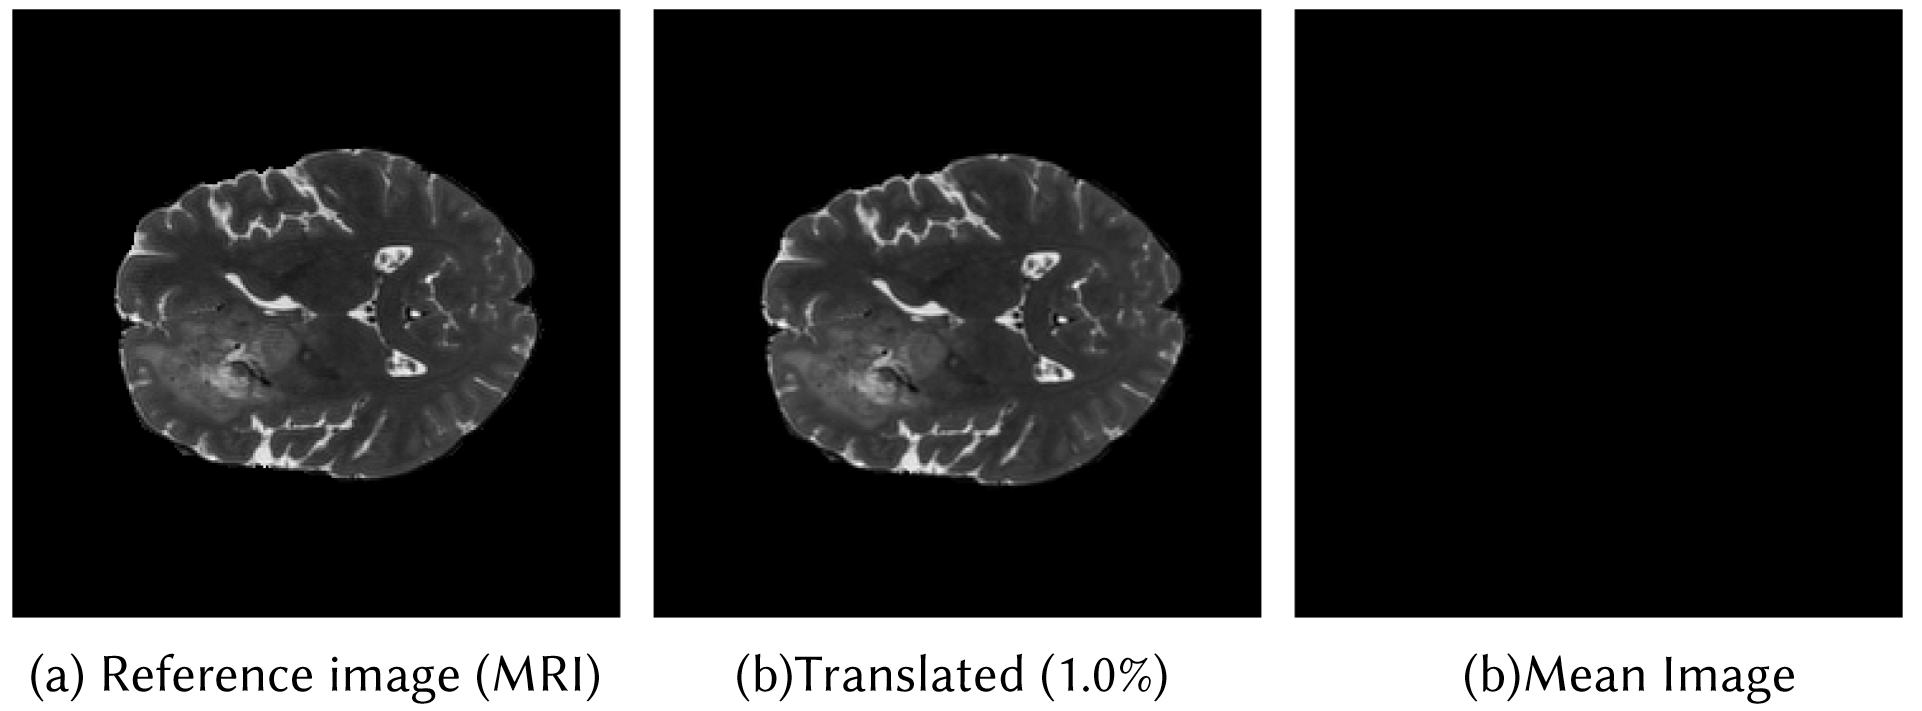
\includegraphics[width=\linewidth]{figures/PSNR_exp.png}
    \caption{The translation experiment. A visually identical translated image suffers massive PSNR degradation compared to the reference.}
    \label{fig:translation_vis}
\end{figure}

As shown in Figure \ref{fig:translation_vis} and detailed in Table \ref{tab:translation_exp}, shifting the image by merely 1.0\% causes the PSNR to plummet drastically to 20.9 dB, a score typically associated with severe degradation. Yet, to the human eye, the 1.0\% translated image is nearly indistinguishable from the reference. In contrast, perceptual metrics like DISTS and LPIPS remain relatively stable and robust to these imperceptible shifts. This experiment definitively proves that purely pixel-aligned metrics like PSNR and MSE heavily penalize slight spatial misalignments while ignoring structural integrity, justifying our critical decision to incorporate Wavelet and Perceptual (LPIPS/DISTS) losses into our final Task 3 pipeline.

\begin{table}[h]
\centering
\caption{Results of the spatial translation experiment on evaluation metrics. Perceptual metrics (DISTS, LPIPS) degrade gracefully, whereas pixel-wise metrics (PSNR, SSIM) collapse under minor shifts.}
\label{tab:translation_exp}
% 使用 resizebox 缩放表格，0.9\linewidth 表示缩放到行宽的 90%
\resizebox{1.0\linewidth}{!}{
\begin{tabular}{lcccc}
\toprule
\textbf{Comparison} & \textbf{DISTS} $\downarrow$ & \textbf{LPIPS} $\downarrow$ & \textbf{PSNR} $\uparrow$ & \textbf{SSIM} $\uparrow$ \\
\midrule
Translated (0.1\%) & 0.028 & 0.007 & 35.9 & 0.988 \\
Translated (1.0\%) & 0.073 & 0.059 & 20.9 & 0.760 \\
Translated (5.0\%) & 0.070 & 0.220 & 17.4 & 0.651 \\
Translated (15.0\%) & 0.120 & 0.422 & 15.2 & 0.538 \\
Mean Image         & 0.655 & 0.612 & 16.8 & 0.085 \\
\bottomrule
\end{tabular}
}
\end{table}

\subsection{Ablation Study}
To validate the individual contributions of our proposed hybrid loss components, we conducted a rigorous ablation study on our network. We incrementally added the Wavelet Loss and the Perceptual (LPIPS) Loss to the baseline MSE objective.


\begin{figure}[h]
    \centering
    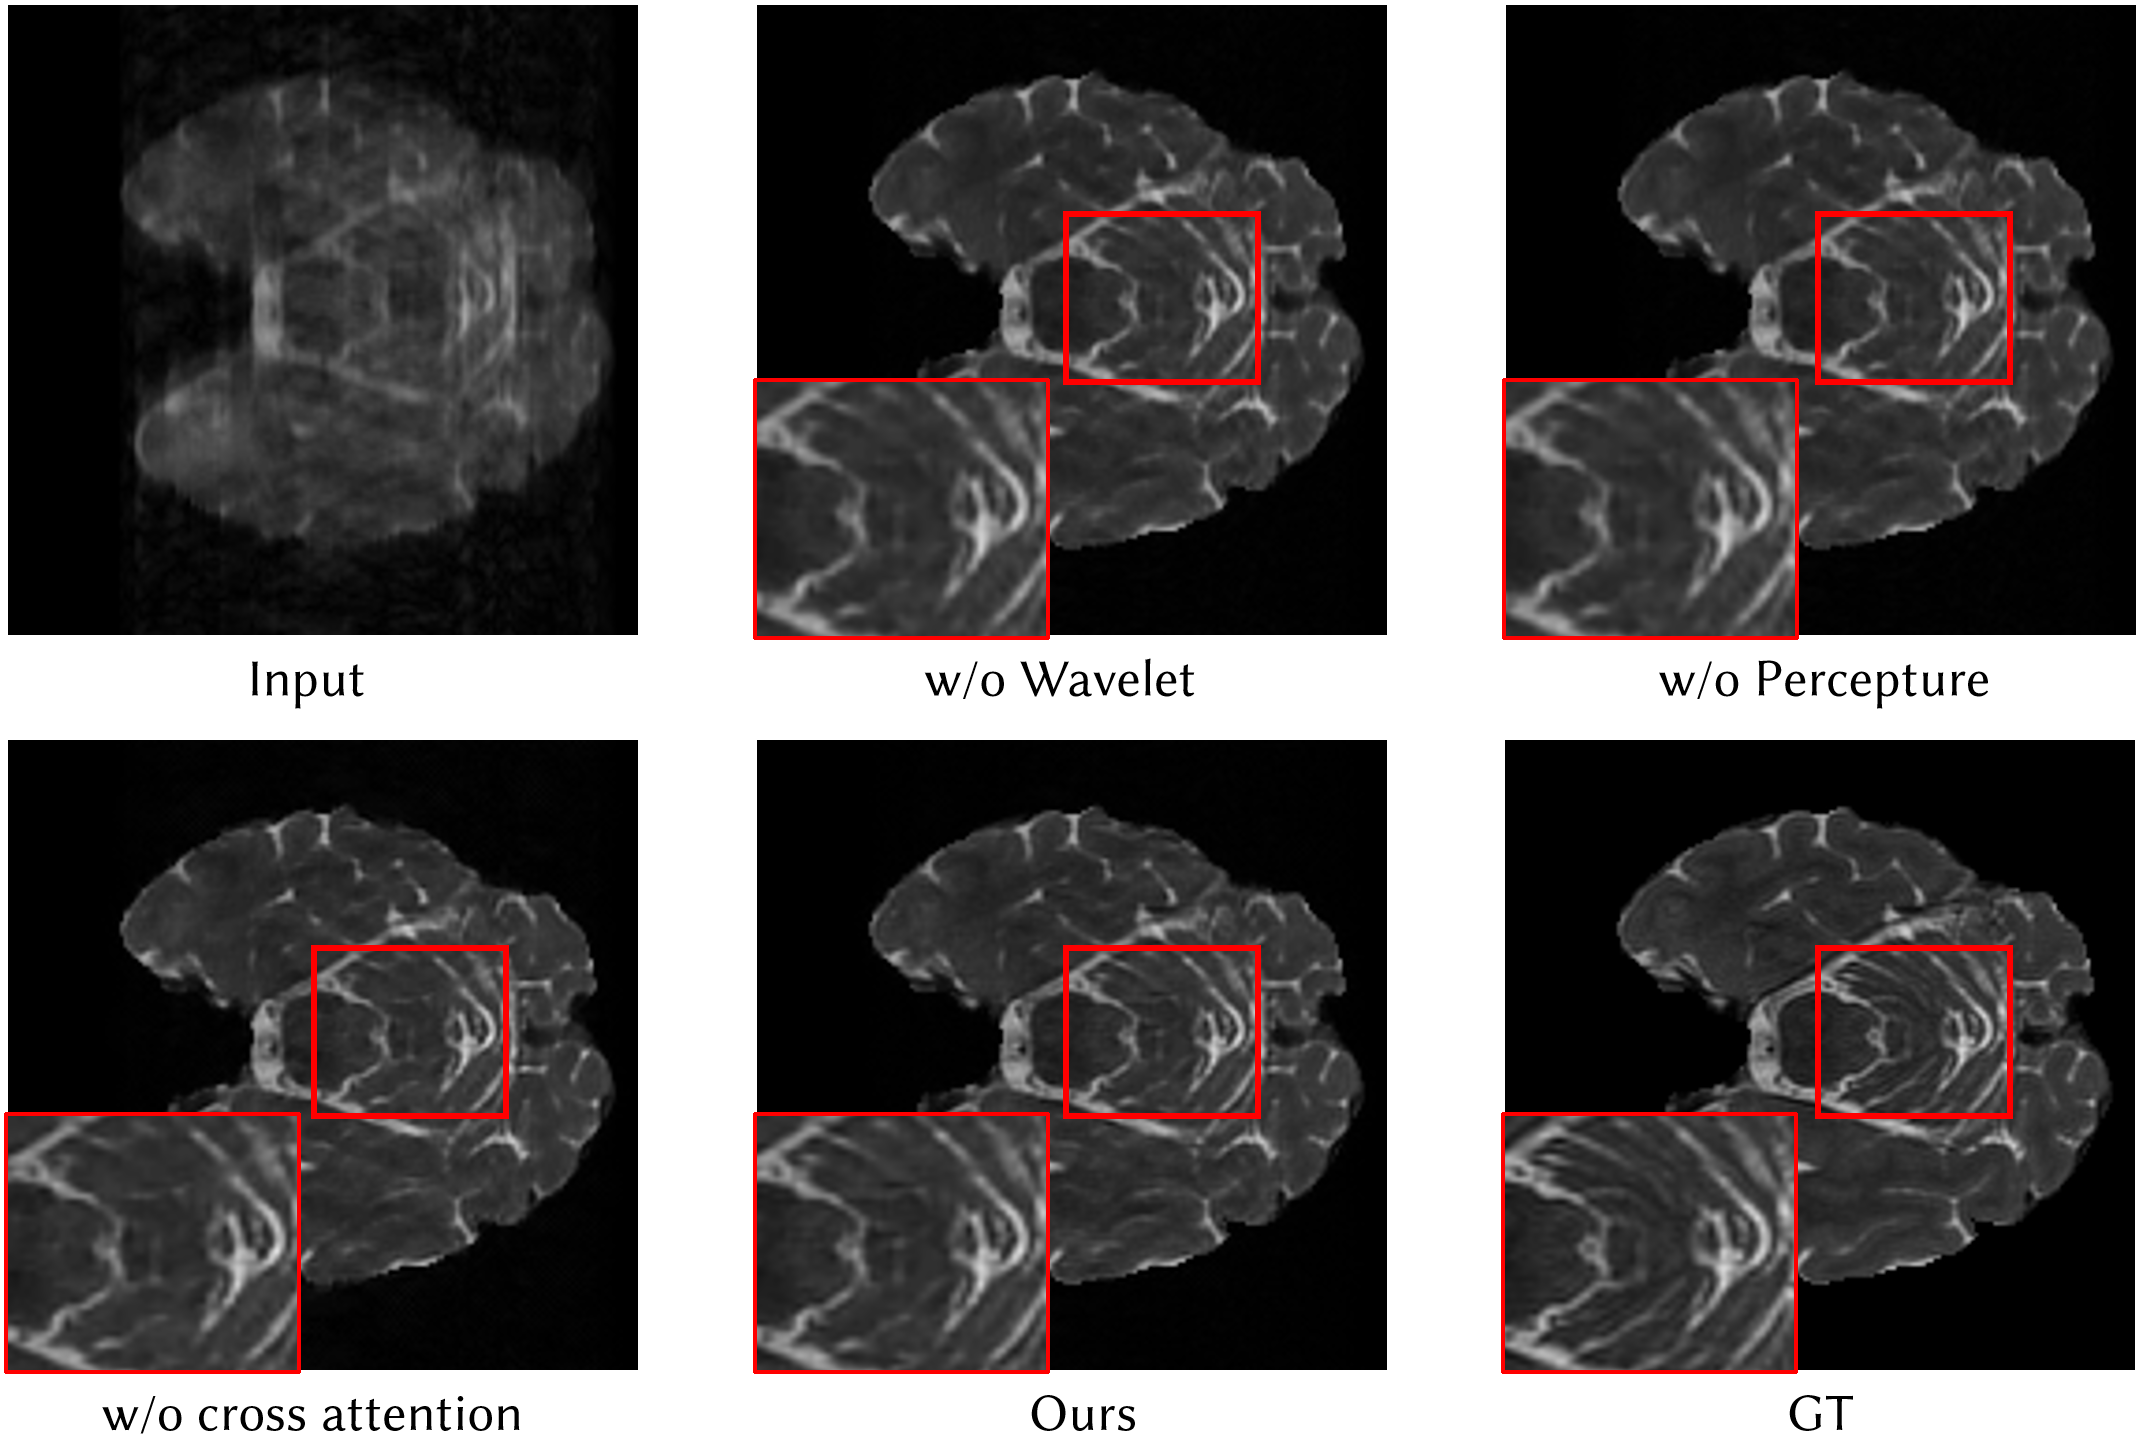
\includegraphics[width=\linewidth]{figures/ablation.png}
    \caption{Qualitative ablation study on key training components.}
    \label{fig:ablation_vis}
\end{figure}

\begin{table}[h]
\centering
\caption{Quantitative ablation results comparing the full proposed multi-modal model against simplified configurations.}
\label{tab:ablation_results}
\resizebox{1.0\linewidth}{!}{
\begin{tabular}{lcccc}
\toprule
\textbf{Configuration} & \textbf{DISTS} $\downarrow$ & \textbf{LPIPS} $\downarrow$ & \textbf{PSNR} $\uparrow$ & \textbf{SSIM} $\uparrow$ \\
\midrule
w/o Wavelet & 0.1289 & 0.0185 & 38.77 & 0.888 \\
w/o Perceptual & 0.1395 & 0.0198 & 37.56 & 0.885 \\
w/o Cross-Attention & 0.1334 & 0.0191 & 37.79 & 0.887 \\
\textbf{Ours (Task 3)} & \textbf{0.0936} & \textbf{0.0090} & \textbf{41.11} & \textbf{0.954} \\
\bottomrule
\end{tabular}
}
\end{table}

As observed in Table \ref{tab:ablation_results} and Figure \ref{fig:ablation_vis}, relying solely on MSE leads to over-smoothed textures. The addition of the Wavelet loss successfully recovers high-frequency edges, while the further integration of the Perceptual loss maximally restores the organic texture of the brain tissues, yielding the best overall DISTS and LPIPS scores.

% \begin{table}[t]
% 	\begin{center}
% 		\centering
% 		\vspace{20pt}

% 		\resizebox{0.47\textwidth}{!}{
% 			\begin{tabular}{l|cccc}
% 				\hline
% 				Method   &  PSNR $\uparrow$ & SSIM $\uparrow$ & LPIPS $\downarrow$ & Training Time(Min / frame) $\downarrow$ \\
% 				\hline
% 				NeuS2~\cite{wang2023neus2}\qquad\qquad & 29.589 & 0.967 & 0.0561 & 3.23  \\
% 			    Spacetime Gaussian~\cite{li2023spacetime}     & 31.691 & 0.981 & 0.0289 & 2.24  \\
%                 DualGS~\cite{jiang2024robust} & \bestCellColor{35.506} & \bestCellColor{0.990} & \secondBestCellColor{0.0193} & 12.22  \\
%                 $V^3$~\cite{wang2024v} & 33.821 & 0.984 & \bestCellColor{0.0167} & \secondBestCellColor{\textbf{1.86}}  \\
%     		\hline
%                 Ours & \secondBestCellColor{\textbf{34.571}} & \secondBestCellColor{\textbf{0.986}} & \textbf{0.0229} & \bestCellColor{\textbf{1.68}} \\
% 				\hline
% 			\end{tabular}
%             }
%             \caption{
%             Quantitative comparison of novel view rendering. Green and yellow cell colors indicate the best and the second-best results. %
%             }
% 		\label{table:Qualitativecomparison}
%         \vspace{-20pt}
% 	\end{center}
% \end{table}

% \begin{table}[t]
%     \centering

%     \resizebox{\columnwidth}{!}{ %
%     \begin{tabular}{c|c c c|c c c}
%         \hline
%         \multirow{2}{*}{\textbf{Methods}} & \multicolumn{3}{c|}{\textbf{Novel View}} & \multicolumn{3}{c}{\textbf{Novel Motion}} \\
%         & PSNR $\uparrow$ & SSIM $\uparrow$  &  LPIPS $\downarrow$ & PSNR $\uparrow$ & SSIM $\uparrow$  &  LPIPS $\downarrow$ \\
%         \hline
%         AP-NeRF ~\cite{uzolas2024template} & 28.26 & 0.939 & 0.0768 & \secondBestCellColor{26.85} & \secondBestCellColor{0.944} & \secondBestCellColor{0.0519} \\
%         TAVA~\cite{li2022tava}  & 21.57 & 0.906 &  0.1292& 21.34 & 0.905 & 0.1301 \\
%         SC-GS~\cite{huang2024sc}  & \secondBestCellColor{30.63} & \secondBestCellColor{0.971} & \secondBestCellColor{0.0319} & 19.18 & 0.907 & 0.0821 \\
%         \hline

%         Ours  & \bestCellColor{\textbf{32.09}} & \bestCellColor{\textbf{0.979}} & \bestCellColor{\textbf{0.0310}} & \bestCellColor{\textbf{30.06}} & \bestCellColor{\textbf{0.976}} & \bestCellColor{\textbf{0.0277}} \\
%         \hline
%     \end{tabular}
%     }
%     \caption{
%     Quantitative comparison with template-free modeling approaches in both novel views and motions. 
%     }
%     \label{table:Qualitativecomparison2}
% \end{table}
